\newpage
%
\section{Appendices}
%
\subsection{Circuit schematics}
%
\vspace{10mm}
%
\begin{multicols}{2}
%
\minipage{\linewidth}
    \begin{center}
        \captionsetup{type=figure}
        \begin{adjustbox}{max width=\linewidth, keepaspectratio}
            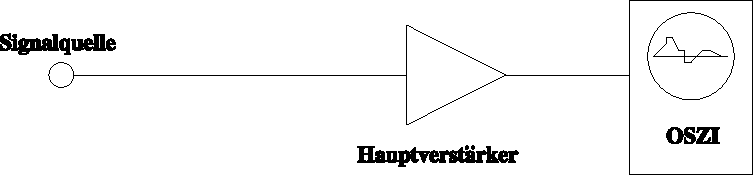
\includegraphics[]{pdf/Schaltung1}
        \end{adjustbox}
        \captionof{figure}{Circuit schematic 1 (Source \cite{Anleitung})}
        \label{fig:Schaltung1}
    \end{center}
\endminipage
%
\vspace{10mm}
%
\minipage{\linewidth}
    \begin{center}
        \captionsetup{type=figure}
        \begin{adjustbox}{max width=\linewidth, keepaspectratio}
            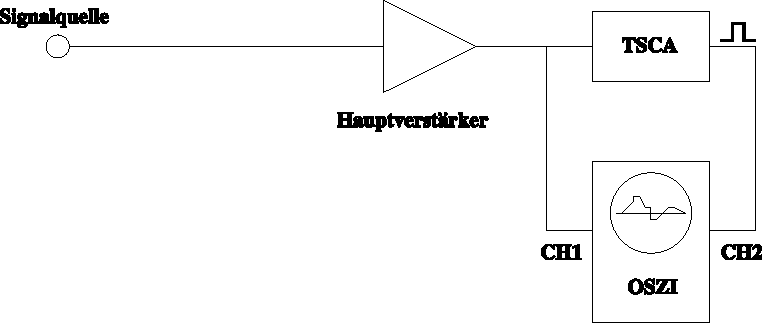
\includegraphics[]{pdf/Schaltung2}
        \end{adjustbox}
        \captionof{figure}{Circuit schematic 2 (Source \cite{Anleitung})}
        \label{fig:Schaltung2}
    \end{center}
\endminipage
%
\vspace{10mm}
%
\minipage{\linewidth}
    \begin{center}
        \captionsetup{type=figure}
        \begin{adjustbox}{max width=\linewidth, keepaspectratio}
            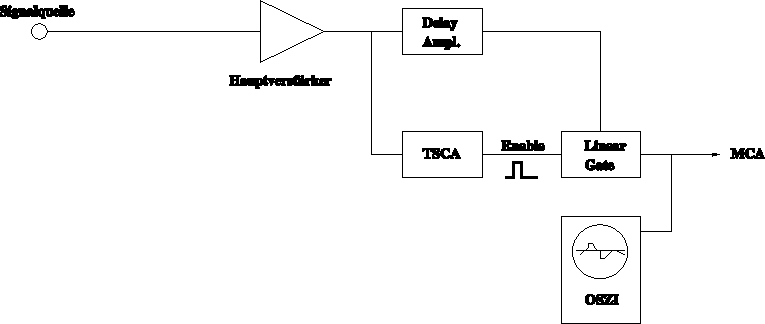
\includegraphics[]{pdf/Schaltung3}
        \end{adjustbox}
        \captionof{figure}{Circuit schematic 3 (Source \cite{Anleitung})}
        \label{fig:Schaltung3}
    \end{center}
\endminipage
%
\vspace{10mm}
%
\minipage{\linewidth}
    \begin{center}
        \captionsetup{type=figure}
        \begin{adjustbox}{max width=\linewidth, keepaspectratio}
            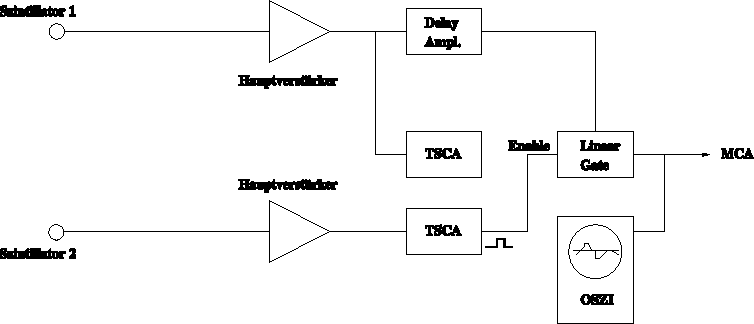
\includegraphics[]{pdf/Schaltung4_mod}
        \end{adjustbox}
        \captionof{figure}{Circuit schematic 4 (Source \cite{Anleitung})}
        \label{fig:Schaltung4}
    \end{center}
\endminipage
%
\vspace{10mm}
%
\minipage{\linewidth}
    \begin{center}
        \captionsetup{type=figure}
        \begin{adjustbox}{max width=\linewidth, keepaspectratio}
            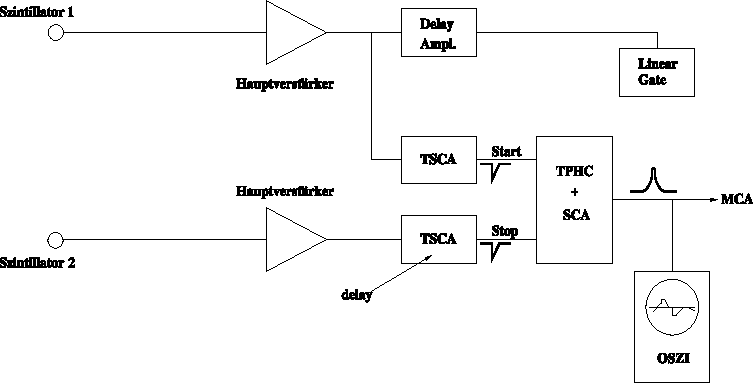
\includegraphics[]{pdf/Schaltung5_mod}
        \end{adjustbox}
        \captionof{figure}{Circuit schematic 5 (Source \cite{Anleitung})}
        \label{fig:Schaltung5}
    \end{center}
\endminipage
%
\vspace{10mm}
%
\minipage{\linewidth}
    \begin{center}
        \captionsetup{type=figure}
        \begin{adjustbox}{max width=\linewidth, keepaspectratio}
            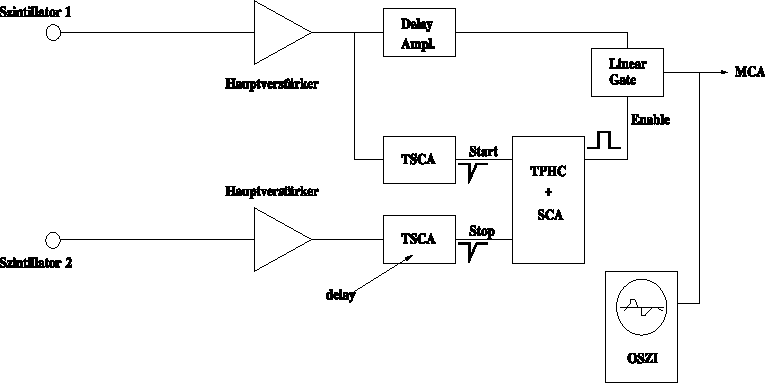
\includegraphics[]{pdf/Schaltung6_mod}
        \end{adjustbox}
        \captionof{figure}{Circuit schematic 6 (Source \cite{Anleitung})}
        \label{fig:Schaltung6}
    \end{center}
\endminipage
%
\newpage
%
\end{multicols}
%
\subsection{Decay schemes}
%
\vspace{10mm}
%
\begin{multicols}{2}
%
\minipage{\linewidth}
    \begin{center}
        \captionsetup{type=figure}
        \begin{adjustbox}{max width=\linewidth, keepaspectratio}
            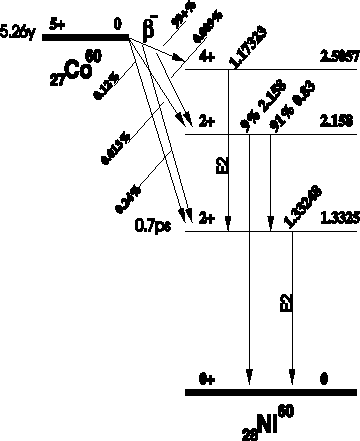
\includegraphics[]{pdf/DecayScheme60Co}
        \end{adjustbox}
        \captionof{figure}{Decay scheme of $^{60}\text{Co}$ (Source \cite{Anleitung})}
        \label{fig:60CoDecayScheme}
    \end{center}
\endminipage
%
\vspace{10mm}
%
\minipage{\linewidth}
    \begin{center}
        \captionsetup{type=figure}
        \begin{adjustbox}{max width=\linewidth, keepaspectratio}
            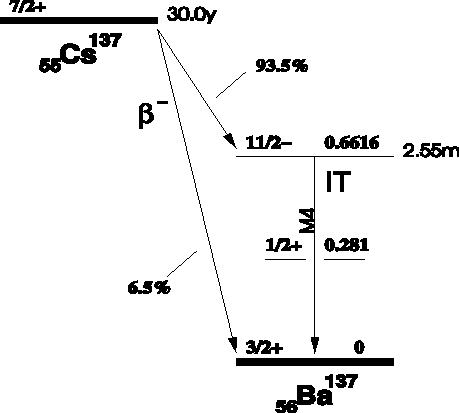
\includegraphics[]{pdf/DecayScheme137Cs}
        \end{adjustbox}
        \captionof{figure}{Decay scheme of $^{137}\text{Cs}$ (Source \cite{Anleitung})}
        \label{fig:137CsDecayScheme}
    \end{center}
\endminipage
%
\vspace{10mm}
%
\minipage{\linewidth}
    \begin{center}
        \captionsetup{type=figure}
        \begin{adjustbox}{max width=\linewidth, keepaspectratio}
            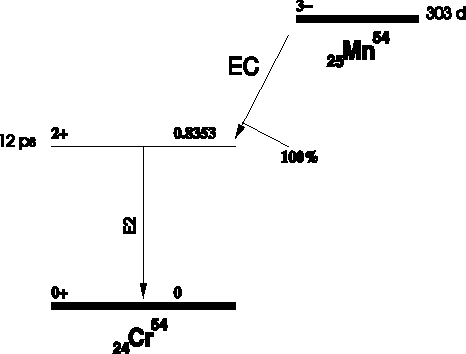
\includegraphics[]{pdf/DecayScheme54Mn}
        \end{adjustbox}
        \captionof{figure}{Decay scheme of $^{54}\text{Mn}$ (Source \cite{Anleitung})}
        \label{fig:54MnDecayScheme}
    \end{center}
\endminipage
%
\vspace{10mm}
%
\minipage{\linewidth}
    \begin{center}
        \captionsetup{type=figure}
        \begin{adjustbox}{max width=\linewidth, keepaspectratio}
            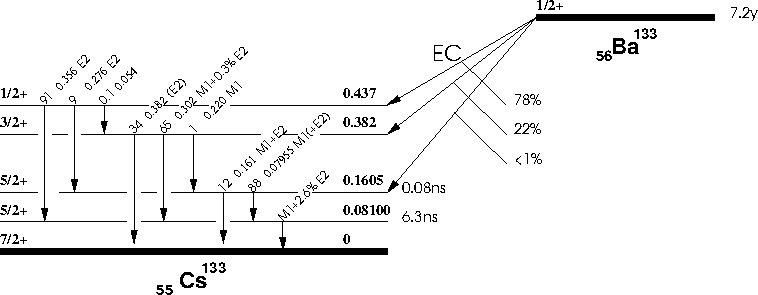
\includegraphics[]{pdf/DecayScheme133Ba}
        \end{adjustbox}
        \captionof{figure}{Decay scheme of $^{133}\text{Ba}$ (Source \cite{Anleitung})}
        \label{fig:133BaDecayScheme}
    \end{center}
\endminipage
%
\vspace{10mm}
%
\minipage{\linewidth}
    \begin{center}
        \captionsetup{type=figure}
        \begin{adjustbox}{max width=\linewidth, keepaspectratio}
            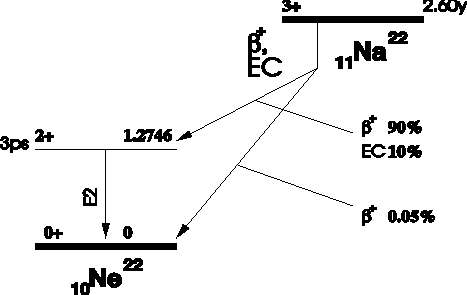
\includegraphics[]{pdf/DecayScheme22Na}
        \end{adjustbox}
        \captionof{figure}{Decay scheme of $^{22}\text{Na}$ (Source \cite{Anleitung})}
        \label{fig:22NaDecayScheme}
    \end{center}
\endminipage
%
\newpage
%
\end{multicols}
%
\subsection{Oscilloscope screenshots}
%
\begin{multicols}{2}
%
\minipage{\linewidth}
    \begin{center}
        \captionsetup{type=figure}
        \begin{adjustbox}{max width=\linewidth, keepaspectratio}
            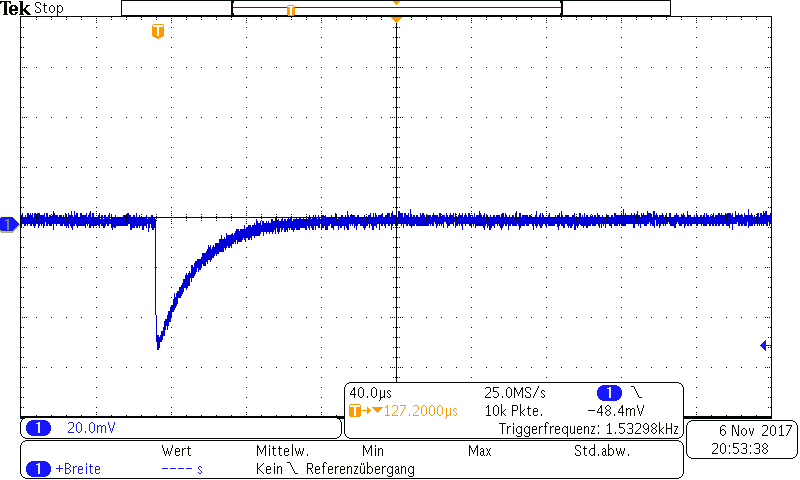
\includegraphics[]{png/tek00000}
        \end{adjustbox}
        \captionof{figure}{Raw signal from detector 1}
        \label{fig:OsciSignal1}
    \end{center}
\endminipage
%
\vspace{10mm}
%
\minipage{\linewidth}
    \begin{center}
        \captionsetup{type=figure}
        \begin{adjustbox}{max width=\linewidth, keepaspectratio}
            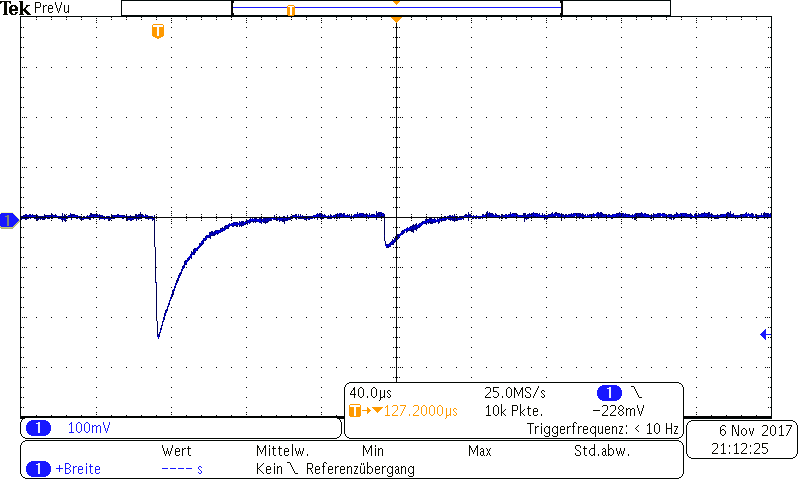
\includegraphics[]{png/tek00001}
        \end{adjustbox}
        \captionof{figure}{Raw signal from detector 2}
        \label{fig:OsciSignal2}
    \end{center}
\endminipage
%
\vspace{10mm}
%
\minipage{\linewidth}
    \begin{center}
        \captionsetup{type=figure}
        \begin{adjustbox}{max width=\linewidth, keepaspectratio}
            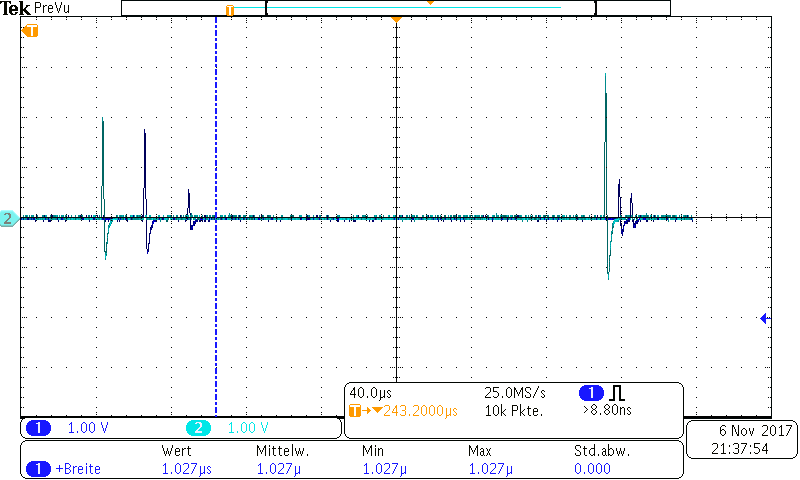
\includegraphics[]{png/tek00003}
        \end{adjustbox}
        \captionof{figure}{Amplified signals from both detectors 1 and 2}
        \label{fig:OsciSignal1and2}
    \end{center}
\endminipage
%
\vspace{10mm}
%
\minipage{\linewidth}
    \begin{center}
        \captionsetup{type=figure}
        \begin{adjustbox}{max width=\linewidth, keepaspectratio}
            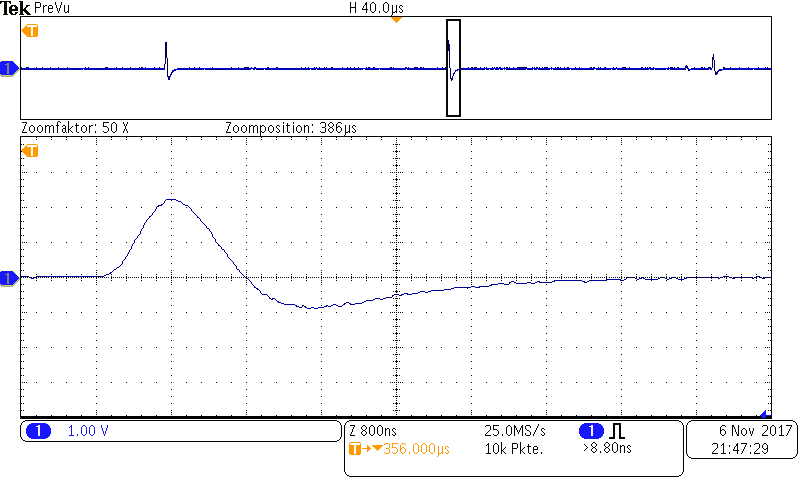
\includegraphics[]{png/tek00004}
        \end{adjustbox}
        \captionof{figure}{Exemplary bipolar signal from detector 1}
        \label{fig:BipolarSignal}
    \end{center}
\endminipage
%
\vspace{10mm}
%
\minipage{\linewidth}
    \begin{center}
        \captionsetup{type=figure}
        \begin{adjustbox}{max width=\linewidth, keepaspectratio}
            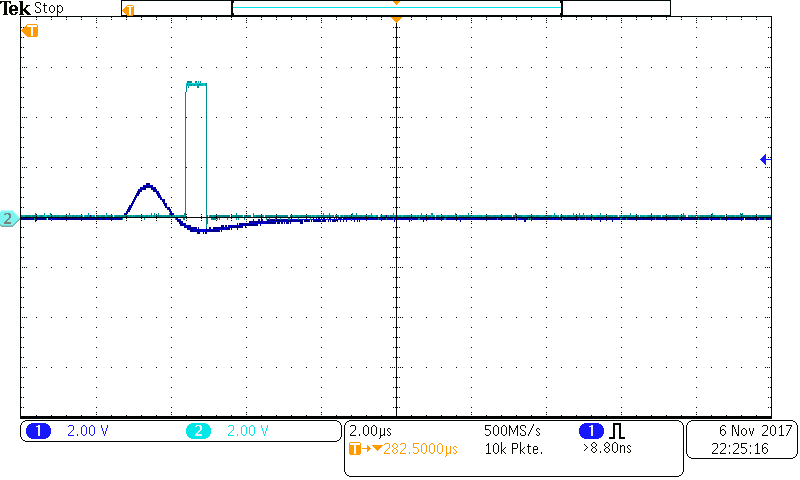
\includegraphics[]{png/tek00006}
        \end{adjustbox}
        \captionof{figure}{Exemplary square wave produced by the TSCA}
        \label{fig:ExampleTSCA}
    \end{center}
\endminipage
%
\vspace{10mm}
%
\minipage{\linewidth}
    \begin{center}
        \captionsetup{type=figure}
        \begin{adjustbox}{max width=\linewidth, keepaspectratio}
            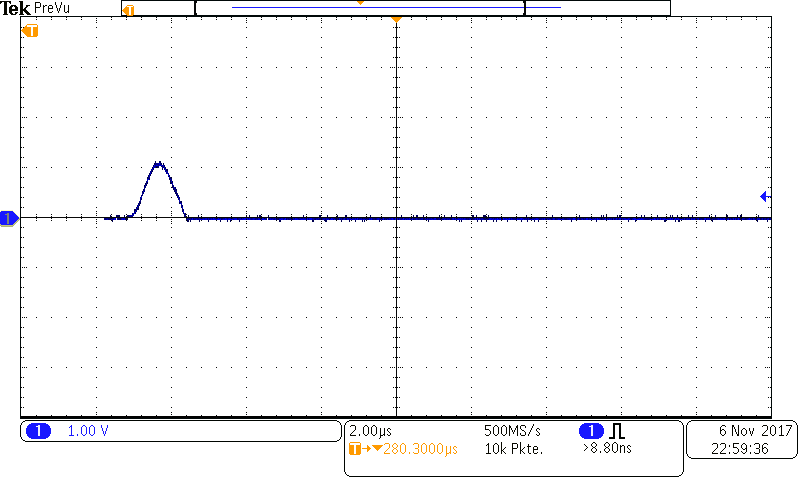
\includegraphics[]{png/tek00007}
        \end{adjustbox}
        \captionof{figure}{TSCA triggers the Linear Gate}
        \label{fig:TSCAplusLG}
    \end{center}
\endminipage
%
\end{multicols}
%
\newpage
%
\subsection{Plots}
%
\begin{multicols}{2}
%
\minipage{\linewidth}
    \begin{center}
        \captionsetup{type=figure}
        \begin{adjustbox}{max width=\linewidth, keepaspectratio}
            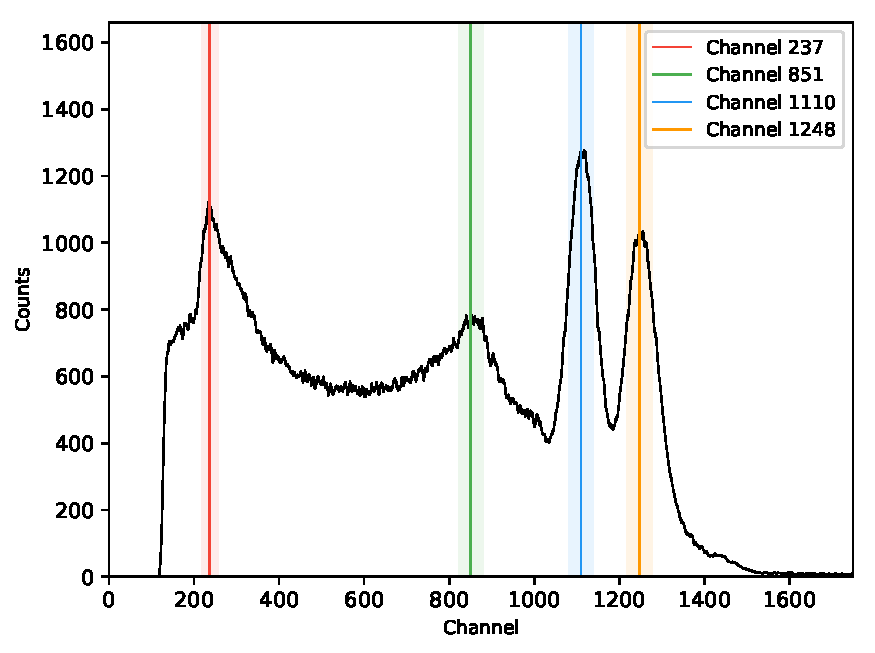
\includegraphics[]{pdf/60Co}
        \end{adjustbox}
        \captionof{figure}{Spectrum of $^{60}\text{Co}$}
        \label{fig:Spectrum60Co}
    \end{center}
\endminipage
%
\vspace{10mm}
%
\minipage{\linewidth}
    \begin{center}
        \captionsetup{type=figure}
        \begin{adjustbox}{max width=\linewidth, keepaspectratio}
            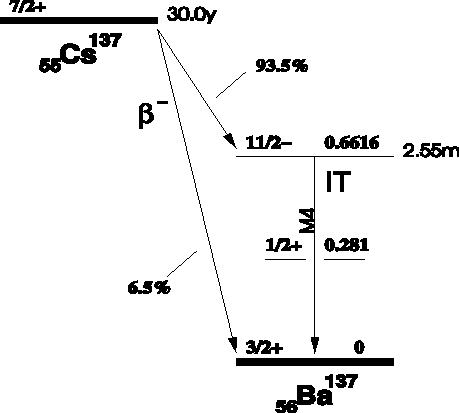
\includegraphics[]{pdf/137Cs}
        \end{adjustbox}
        \captionof{figure}{Spectrum of $^{137}\text{Cs}$}
        \label{fig:Spectrum137Cs}
    \end{center}
\endminipage
%
\vspace{10mm}
%
\minipage{\linewidth}
    \begin{center}
        \captionsetup{type=figure}
        \begin{adjustbox}{max width=\linewidth, keepaspectratio}
            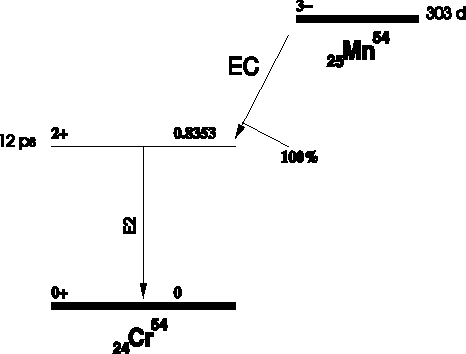
\includegraphics[]{pdf/54Mn}
        \end{adjustbox}
        \captionof{figure}{Spectrum of $^{54}\text{Mn}$}
        \label{fig:Spectrum54Mn}
    \end{center}
\endminipage
%
\vspace{10mm}
%
\minipage{\linewidth}
    \begin{center}
        \captionsetup{type=figure}
        \begin{adjustbox}{max width=\linewidth, keepaspectratio}
            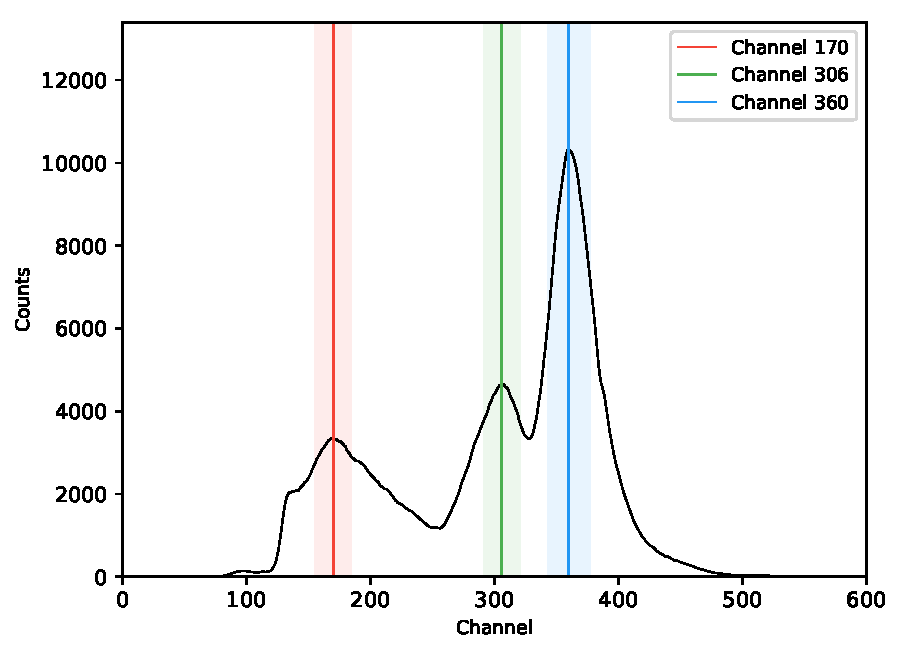
\includegraphics[]{pdf/133Ba}
        \end{adjustbox}
        \captionof{figure}{Spectrum of $^{133}\text{Ba}$}
        \label{fig:Spectrum133Ba}
    \end{center}
\endminipage
%
\vspace{10mm}
%
\minipage{\linewidth}
    \begin{center}
        \captionsetup{type=figure}
        \begin{adjustbox}{max width=\linewidth, keepaspectratio}
            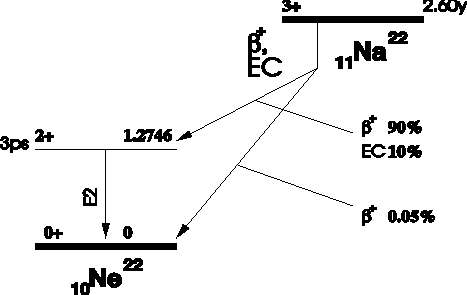
\includegraphics[]{pdf/22Na}
        \end{adjustbox}
        \captionof{figure}{Spectrum of $^{22}\text{Na}$}
        \label{fig:Spectrum22Na}
    \end{center}
\endminipage
%
\vspace{10mm}
%
\minipage{\linewidth}
    \begin{center}
        \captionsetup{type=figure}
        \begin{adjustbox}{max width=\linewidth, keepaspectratio}
            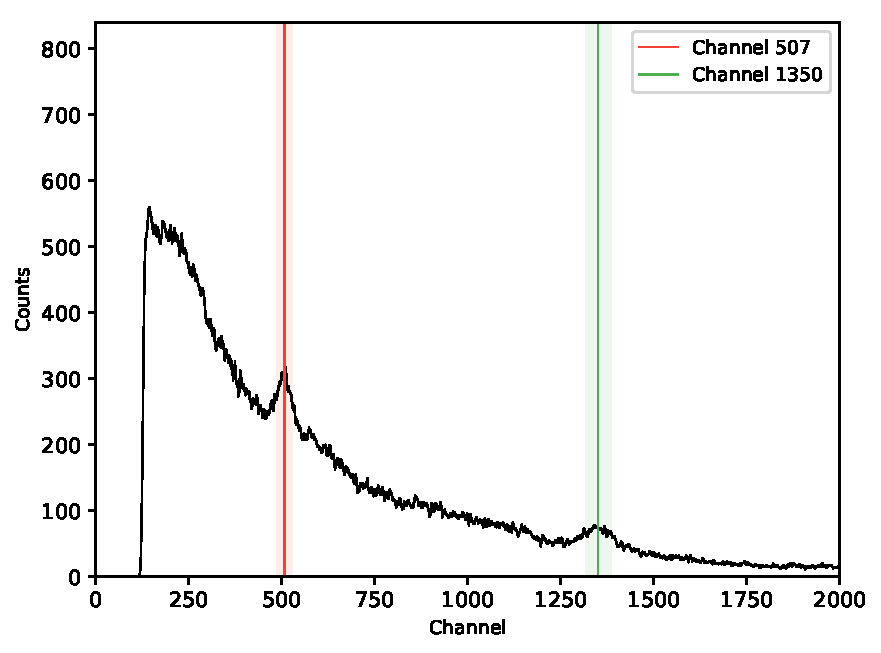
\includegraphics[]{pdf/night}
        \end{adjustbox}
        \captionof{figure}{Spectrum of night measurement}
        \label{fig:SpectrumNight}
    \end{center}
\endminipage
%
\vspace{10mm}
%
\minipage{\linewidth}
    \begin{center}
        \captionsetup{type=figure}
        \begin{adjustbox}{max width=\linewidth, keepaspectratio}
            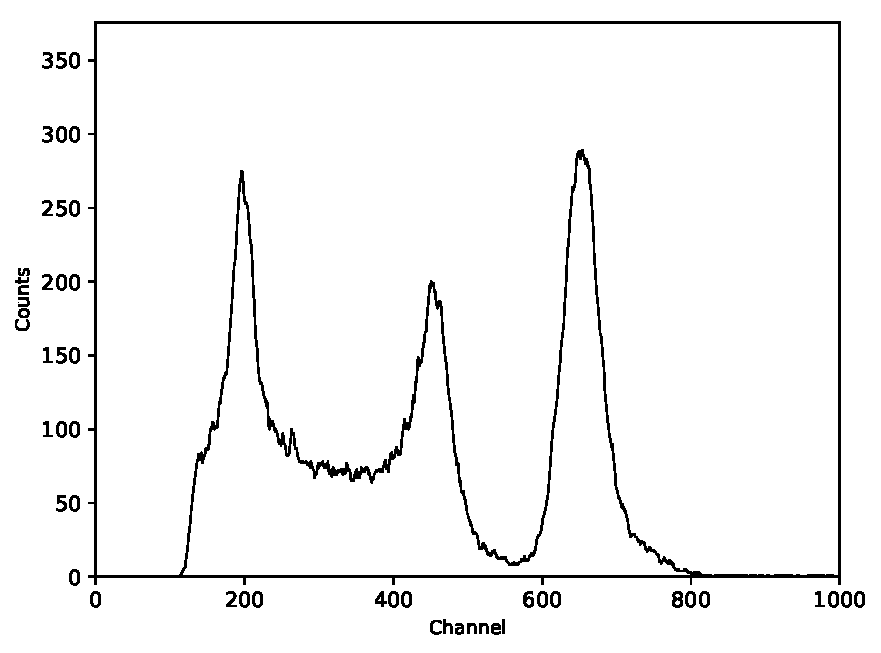
\includegraphics[]{pdf/137Cskoinz1}
        \end{adjustbox}
        \captionof{figure}{Spectrum of $^{137}\text{Cs}$ with simple coincidence setup}
        \label{fig:137Cskoinz1}
    \end{center}
\endminipage
%
\vspace{10mm}
%
\minipage{\linewidth}
    \begin{center}
        \captionsetup{type=figure}
        \begin{adjustbox}{max width=\linewidth, keepaspectratio}
            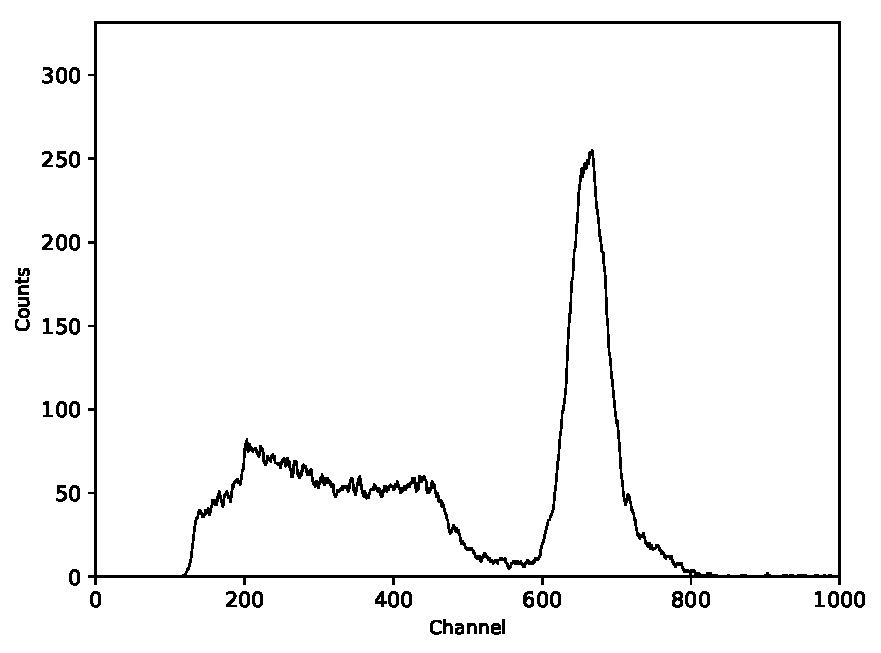
\includegraphics[]{pdf/137Cskoinz2}
        \end{adjustbox}
        \captionof{figure}{Random coincidence spectrum of $^{137}\text{Cs}$}
        \label{fig:137Cskoinz2}
    \end{center}
\endminipage
%
\vspace{10mm}
%
\minipage{\linewidth}
    \begin{center}
        \captionsetup{type=figure}
        \begin{adjustbox}{max width=\linewidth, keepaspectratio}
            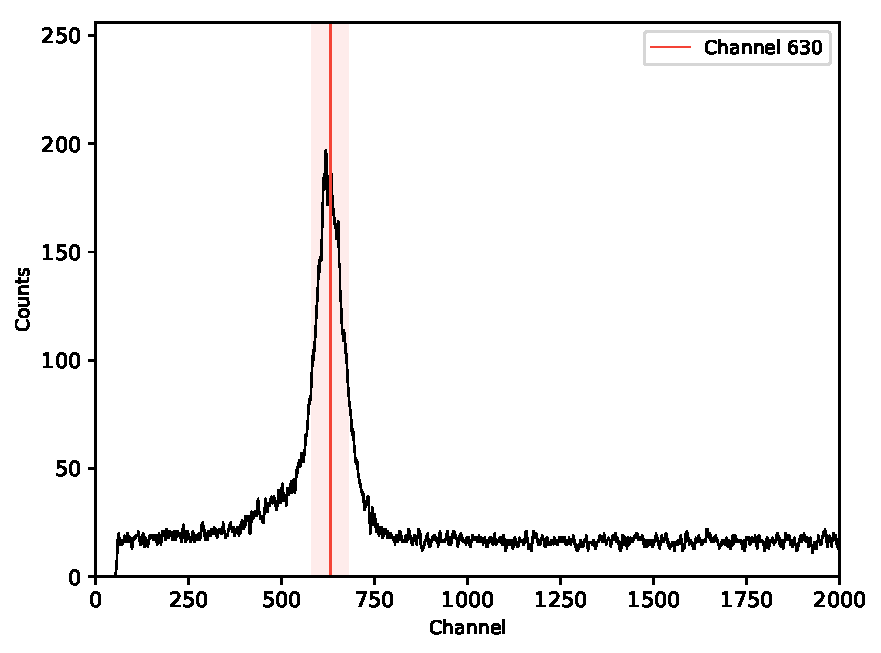
\includegraphics[]{pdf/137CsTPHC}
        \end{adjustbox}
        \captionof{figure}{Time spectrum of $^{137}\text{Cs}$}
        \label{fig:137CsTPHC}
    \end{center}
\endminipage
%
\vspace{10mm}
%
\minipage{\linewidth}
    \begin{center}
        \captionsetup{type=figure}
        \begin{adjustbox}{max width=\linewidth, keepaspectratio}
            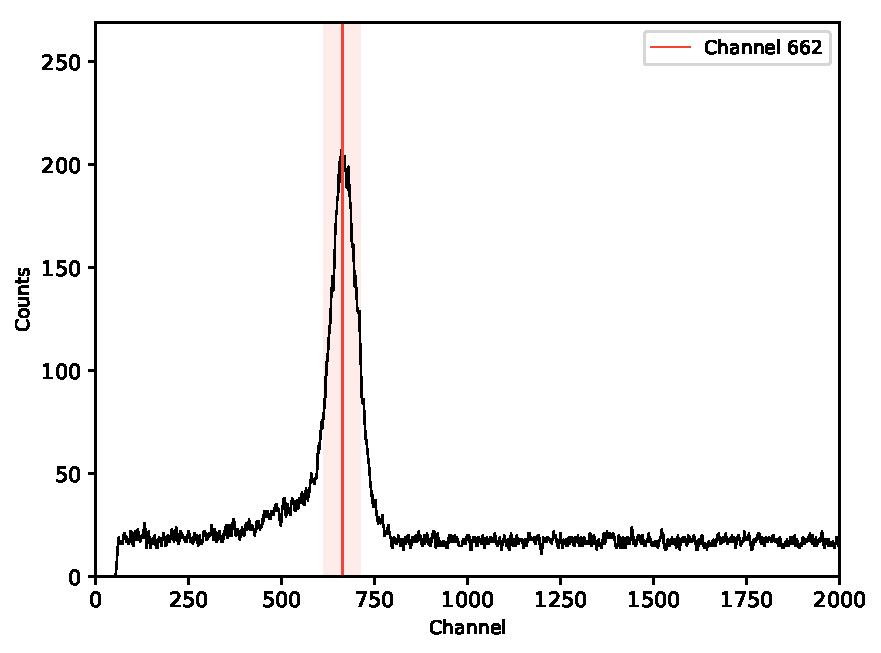
\includegraphics[]{pdf/137CsTPHC20ns}
        \end{adjustbox}
        \captionof{figure}{Time spectrum of $^{137}\text{Cs}$ with \SI{20}{\nano\second} delay}
        \label{fig:137CsTPHC20ns}
    \end{center}
\endminipage
%
\vspace{10mm}
%
\minipage{\linewidth}
    \begin{center}
        \captionsetup{type=figure}
        \begin{adjustbox}{max width=\linewidth, keepaspectratio}
            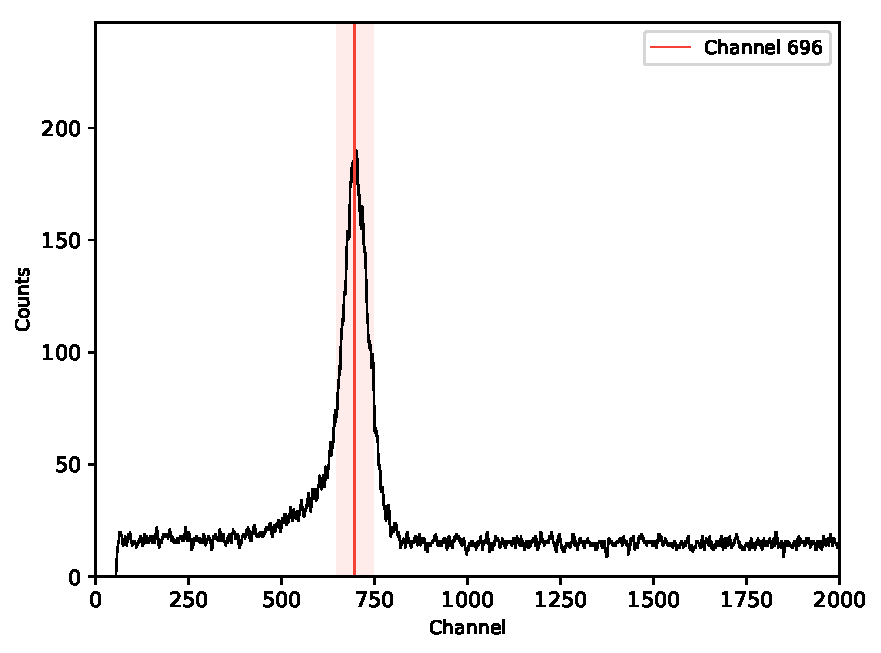
\includegraphics[]{pdf/137CsTPHC40ns}
        \end{adjustbox}
        \captionof{figure}{Time spectrum of $^{137}\text{Cs}$ with \SI{40}{\nano\second} delay}
        \label{fig:137CsTPHC40ns}
    \end{center}
\endminipage
%
\vspace{10mm}
%
\minipage{\linewidth}
    \begin{center}
        \captionsetup{type=figure}
        \begin{adjustbox}{max width=\linewidth, keepaspectratio}
            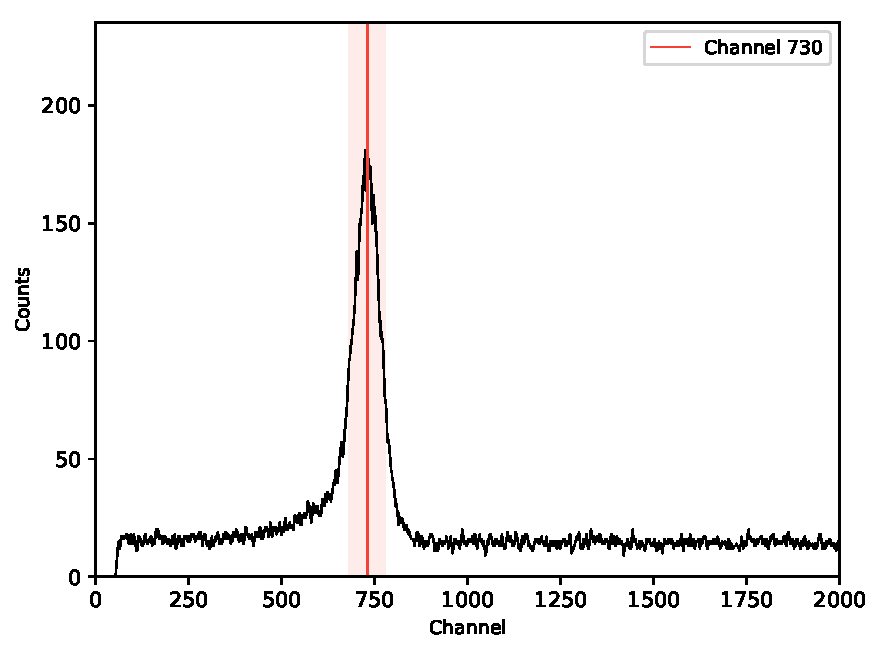
\includegraphics[]{pdf/137CsTPHC60ns}
        \end{adjustbox}
        \captionof{figure}{Time spectrum of $^{137}\text{Cs}$ with \SI{60}{\nano\second} delay}
        \label{fig:137CsTPHC60ns}
    \end{center}
\endminipage
%
\vspace{10mm}
%
\minipage{\linewidth}
    \begin{center}
        \captionsetup{type=figure}
        \begin{adjustbox}{max width=\linewidth, keepaspectratio}
            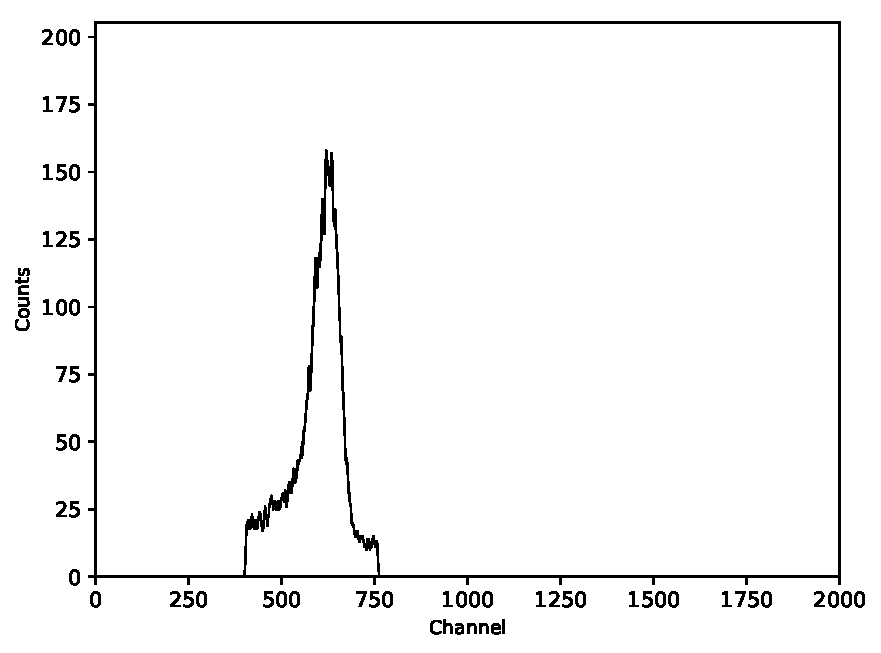
\includegraphics[]{pdf/137CsTPHC_geschnitten_neu}
        \end{adjustbox}
        \captionof{figure}{Time spectrum of $^{137}\text{Cs}$ cut to coincidence peak}
        \label{fig:137CsTPHC_geschnitten_neu}
    \end{center}
\endminipage
%
\vspace{10mm}
%
\minipage{\linewidth}
    \begin{center}
        \captionsetup{type=figure}
        \begin{adjustbox}{max width=\linewidth, keepaspectratio}
            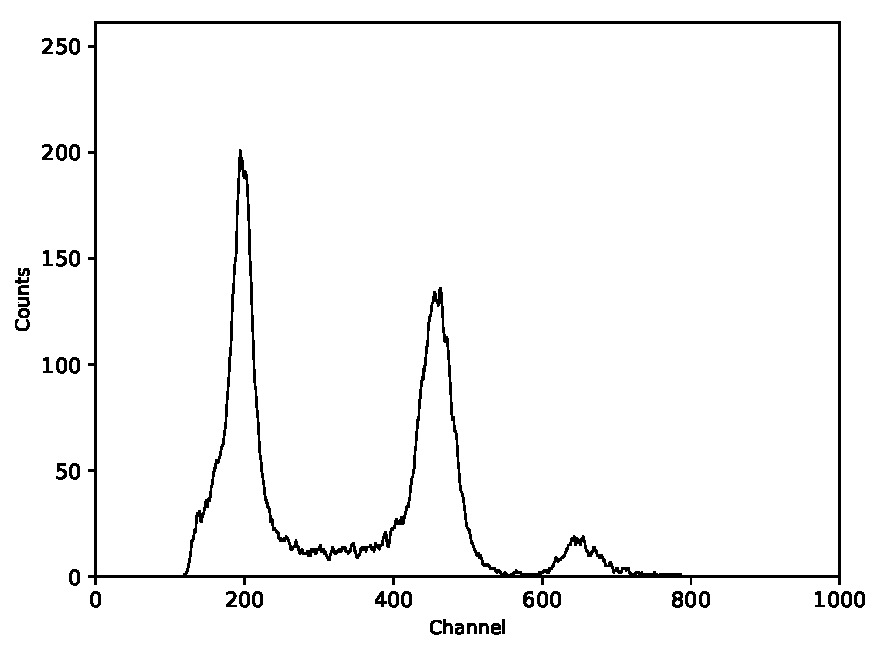
\includegraphics[]{pdf/137CsmitTPHC_gated}
        \end{adjustbox}
        \captionof{figure}{Spectrum of $^{137}\text{Cs}$ with time window}
        \label{fig:137CsmitTPHC_gated}
    \end{center}
\endminipage
%
\vspace{10mm}
%
\minipage{\linewidth}
    \begin{center}
        \captionsetup{type=figure}
        \begin{adjustbox}{max width=\linewidth, keepaspectratio}
            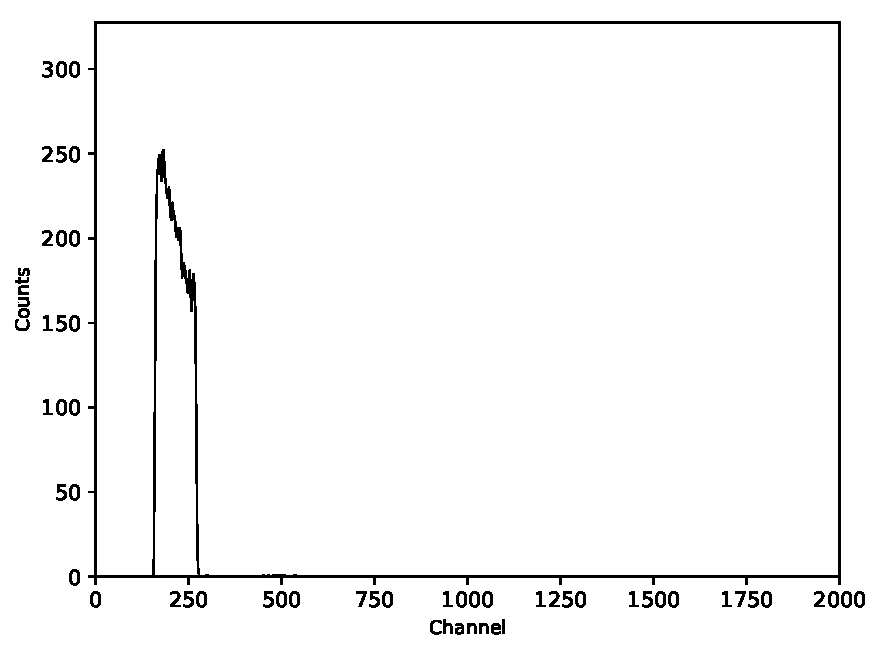
\includegraphics[]{pdf/signal2eneriewindow}
        \end{adjustbox}
        \captionof{figure}{Spectrum of $^{137}\text{Cs}$ at detector 2 with energy window}
        \label{fig:signal2eneriewindow}
    \end{center}
\endminipage
%
\vspace{10mm}
%
\minipage{\linewidth}
    \begin{center}
        \captionsetup{type=figure}
        \begin{adjustbox}{max width=\linewidth, keepaspectratio}
            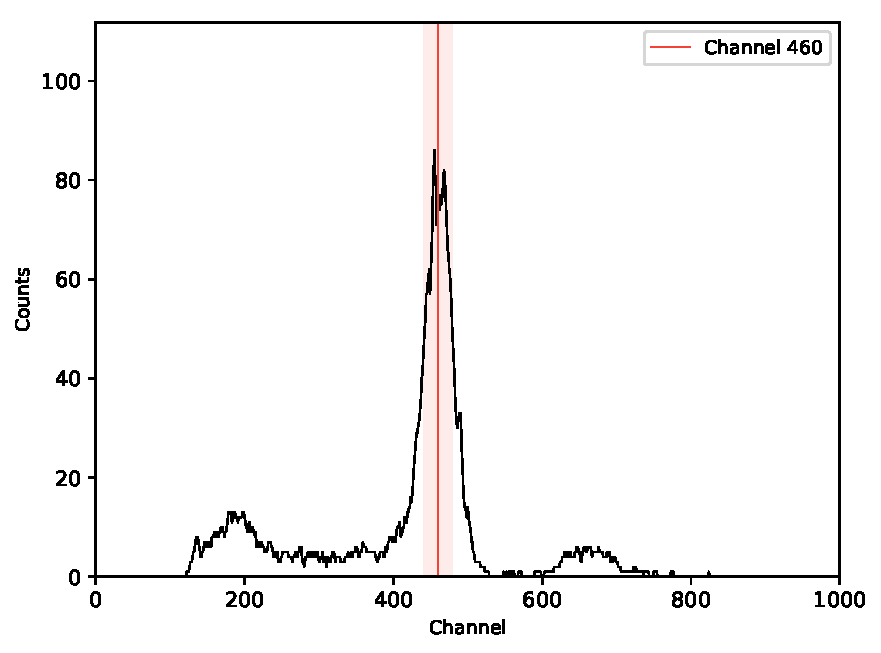
\includegraphics[]{pdf/comptonpeak}
        \end{adjustbox}
        \captionof{figure}{Spectrum of $^{137}\text{Cs}$ with time and energy window}
        \label{fig:comptonpeak}
    \end{center}
\endminipage
%
\vspace{10mm}
%
\minipage{\linewidth}
    \begin{center}
        \captionsetup{type=figure}
        \begin{adjustbox}{max width=\linewidth, keepaspectratio}
            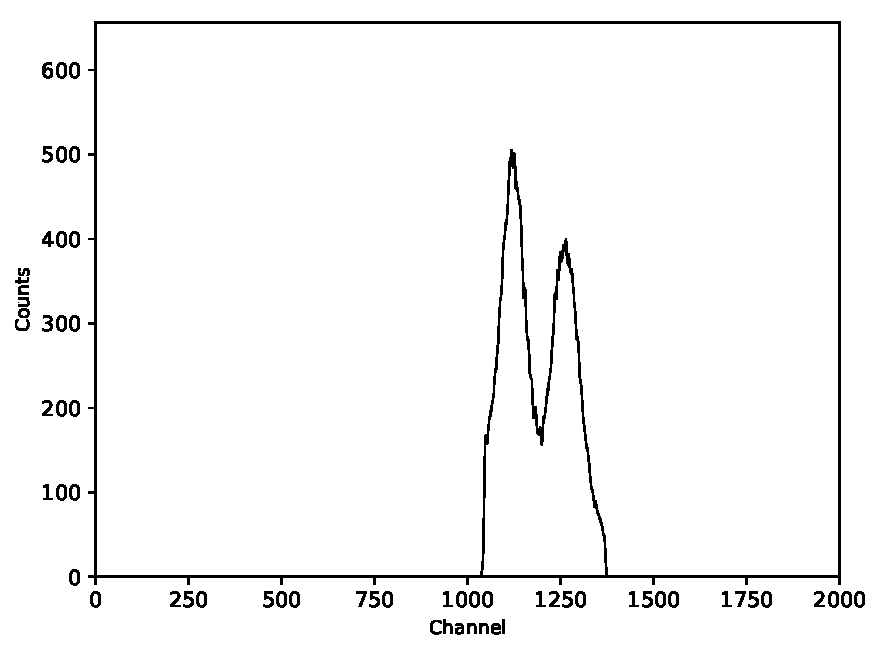
\includegraphics[]{pdf/60CoEnergiewindow1}
        \end{adjustbox}
        \captionof{figure}{Spectrum of $^{60}\text{Co}$ at detector 1 with energy window}
        \label{fig:60CoEnergiewindow1}
    \end{center}
\endminipage
%
\vspace{10mm}
%
\minipage{\linewidth}
    \begin{center}
        \captionsetup{type=figure}
        \begin{adjustbox}{max width=\linewidth, keepaspectratio}
            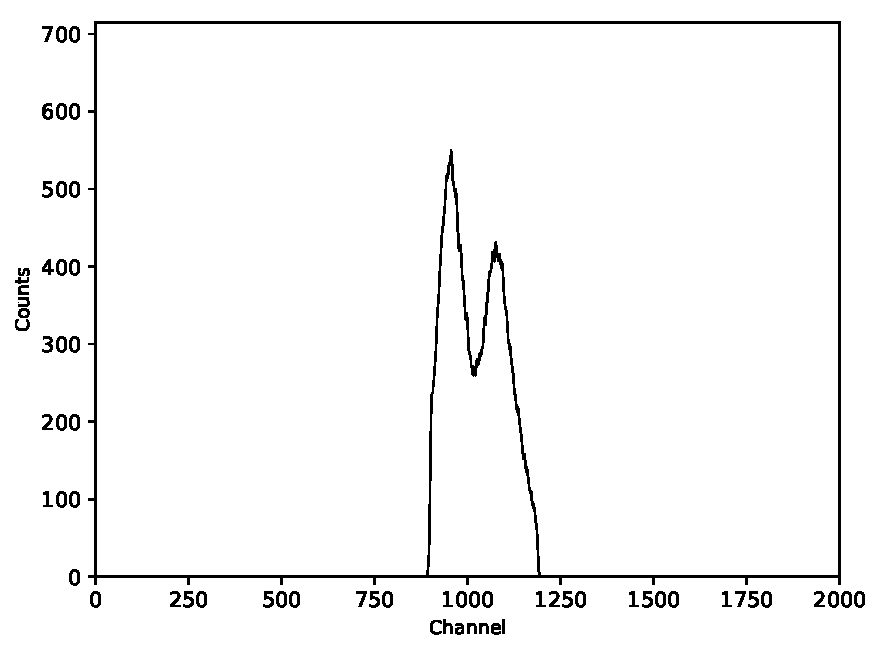
\includegraphics[]{pdf/60CoEnergiewindow2}
        \end{adjustbox}
        \captionof{figure}{Spectrum of $^{60}\text{Co}$ at detector 2 with energy window}
        \label{fig:60CoEnergiewindow2}
    \end{center}
\endminipage
%
\vspace{10mm}
%
\minipage{\linewidth}
    \begin{center}
        \captionsetup{type=figure}
        \begin{adjustbox}{max width=\linewidth, keepaspectratio}
            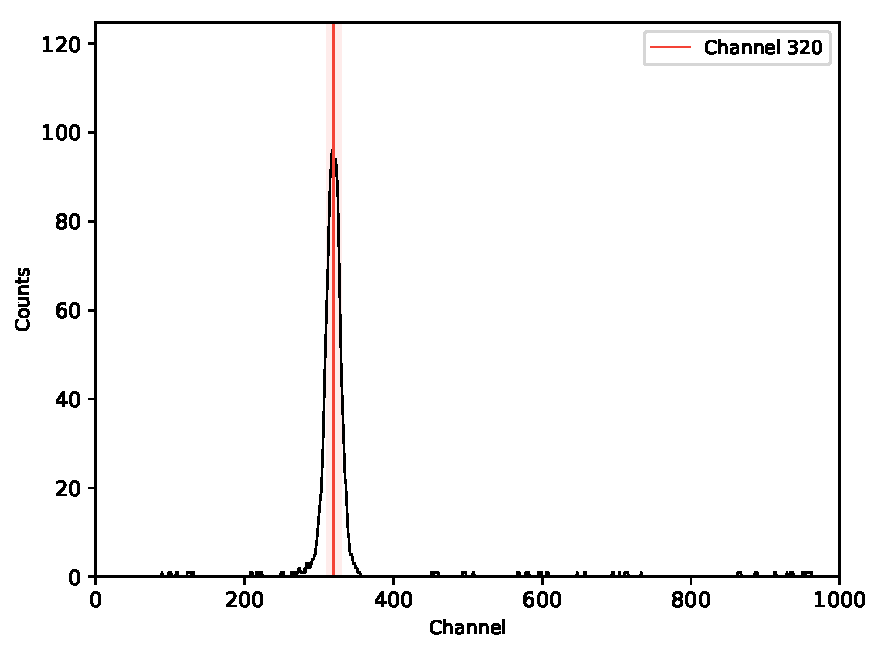
\includegraphics[]{pdf/60CoZeitspektrum}
        \end{adjustbox}
        \captionof{figure}{Time spectrum of $^{60}\text{Co}$}
        \label{fig:60CoZeitspektrum}
    \end{center}
\endminipage
%
\vspace{10mm}
%
\minipage{\linewidth}
    \begin{center}
        \captionsetup{type=figure}
        \begin{adjustbox}{max width=\linewidth, keepaspectratio}
            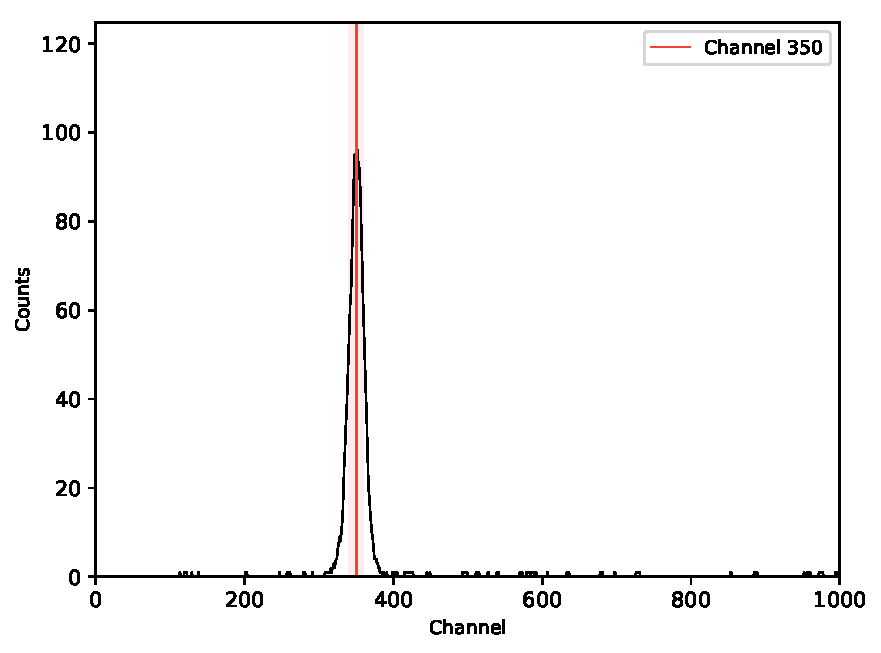
\includegraphics[]{pdf/60CoZeitspektrum20ns}
        \end{adjustbox}
        \captionof{figure}{Time spectrum of $^{60}\text{Co}$ with \SI{20}{\nano\second} delay}
        \label{fig:60CoZeitspektrum20ns}
    \end{center}
\endminipage
%
\vspace{10mm}
%
\minipage{\linewidth}
    \begin{center}
        \captionsetup{type=figure}
        \begin{adjustbox}{max width=\linewidth, keepaspectratio}
            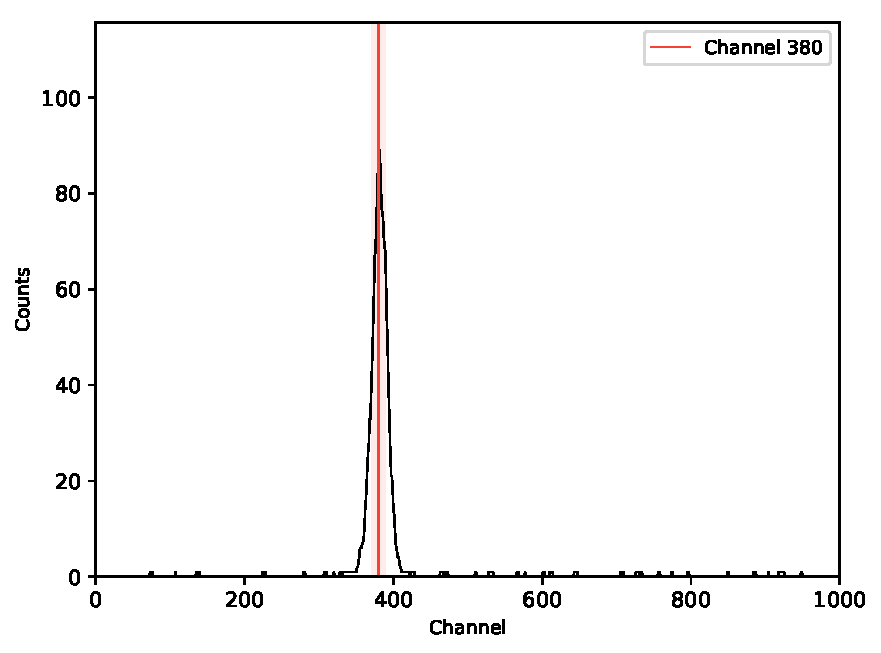
\includegraphics[]{pdf/60CoZeitspektrum40ns}
        \end{adjustbox}
        \captionof{figure}{Time spectrum of $^{60}\text{Co}$ with \SI{40}{\nano\second} delay}
        \label{fig:60CoZeitspektrum40ns}
    \end{center}
\endminipage
%
\vspace{10mm}
%
\minipage{\linewidth}
    \begin{center}
        \captionsetup{type=figure}
        \begin{adjustbox}{max width=\linewidth, keepaspectratio}
            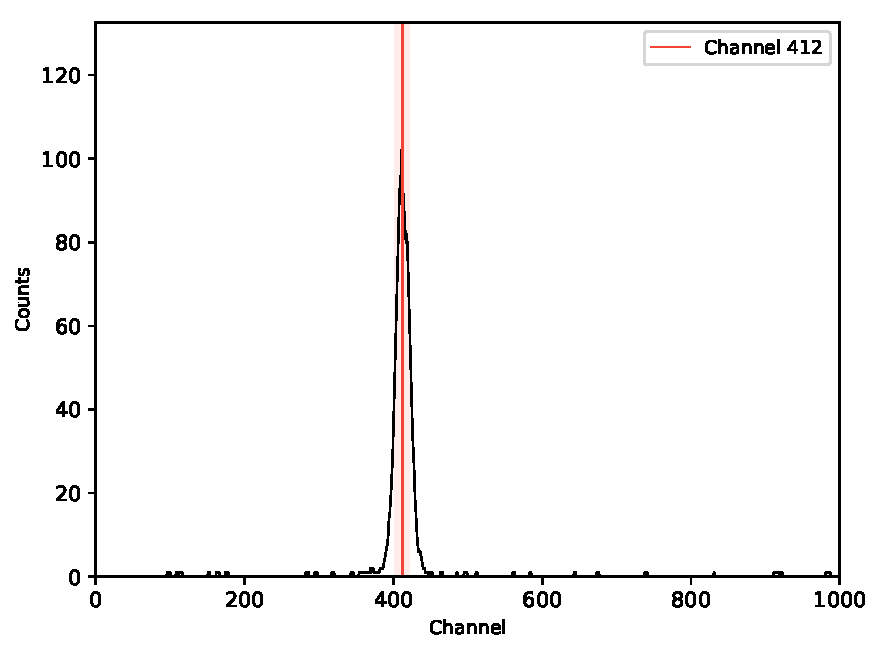
\includegraphics[]{pdf/60CoZeitspektrum60ns}
        \end{adjustbox}
        \captionof{figure}{Time spectrum of $^{60}\text{Co}$ with \SI{60}{\nano\second} delay}
        \label{fig:60CoZeitspektrum60ns}
    \end{center}
\endminipage
%
\vspace{10mm}
%
\minipage{\linewidth}
    \begin{center}
        \captionsetup{type=figure}
        \begin{adjustbox}{max width=\linewidth, keepaspectratio}
            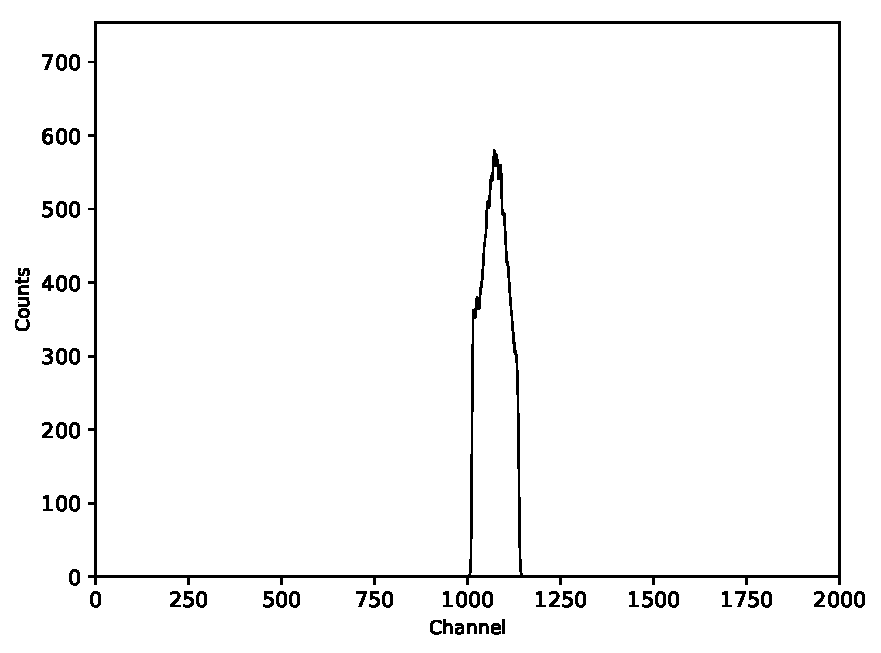
\includegraphics[]{pdf/60CoEnergiewindow2-peak2}
        \end{adjustbox}
        \captionof{figure}{Spectrum of $^{60}\text{Co}$ at detector 2 with energy window around peak 2}
        \label{fig:60CoEnergiewindow2-peak2}
    \end{center}
\endminipage
%
\vspace{10mm}
%
\minipage{\linewidth}
    \begin{center}
        \captionsetup{type=figure}
        \begin{adjustbox}{max width=\linewidth, keepaspectratio}
            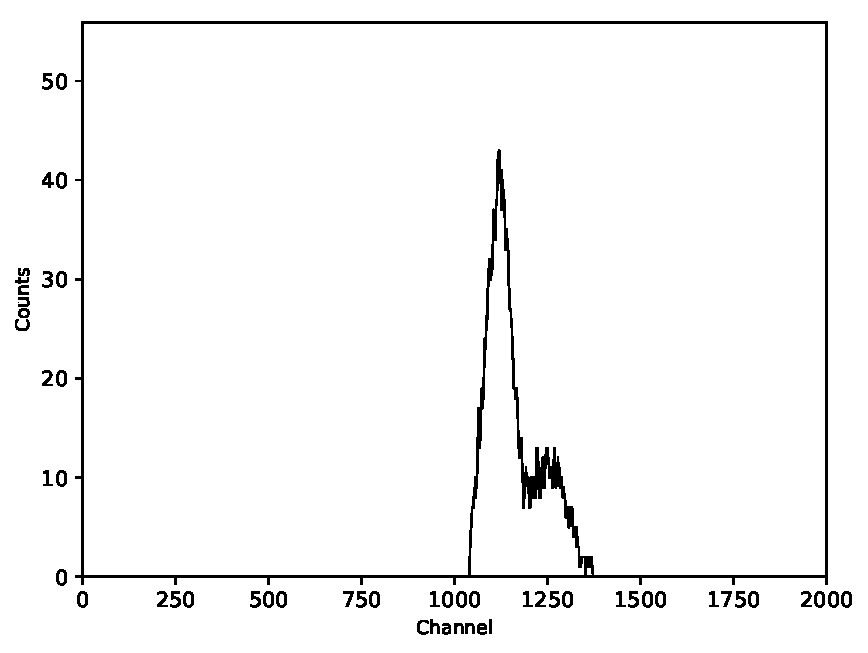
\includegraphics[]{pdf/60CoKaskadenEnergiewindowBeiPeak2}
        \end{adjustbox}
        \captionof{figure}{Spectrum of $^{60}\text{Co}$ showing coincidence}
        \label{fig:60CoKaskadenEnergiewindowBeiPeak2}
    \end{center}
\endminipage
%
\end{multicols}
%
